\documentclass[conference]{IEEEtran}
\usepackage{cite}
\usepackage{amsmath,amssymb,amsfonts}
\usepackage{algorithmic}
\usepackage{graphicx}
\usepackage{textcomp}
\usepackage{xcolor}
\usepackage{pgfplots}
\pgfplotsset{compat=1.18}

\usepackage{tikz}
\usetikzlibrary{arrows.meta, positioning, shapes.geometric}
\usepackage{pagecolor}

% add for full-width equations in two-column layout
\usepackage{cuted}      % provides strip environment for full-width equations
\usepackage{stfloats}   % improved placement for figure*/table* floats

% Define a very gentle pastel green for the background
\definecolor{gentlegreen}{RGB}{245, 252, 245}
\pagecolor{gentlegreen}

% Hyperref package for PDF bookmarks and outlines
\usepackage[bookmarks=true,
            bookmarksnumbered=true,
            bookmarksopen=true,
            bookmarksopenlevel=2,
            pdfborder={0 0 0},
            pdfstartview=FitH,
            pdftitle={The Calçotada Protocol: Equity Peg Tokens for Decentralized Venture Capital},
            pdfauthor={Dr. Julià Delos Ayllón},
            pdfsubject={Blockchain-based Venture Capital Protocol},
            pdfkeywords={Blockchain, Venture Capital, Decentralized Finance, Tokenization, Equity Peg Token, DAO},
            colorlinks=true,
            linkcolor=black,
            citecolor=black,
            urlcolor=blue,
            filecolor=black]{hyperref}
\usepackage{bookmark} % Enhanced bookmark handling

\begin{document}

% Force page numbers to appear
\thispagestyle{plain}
\pagestyle{plain}

\title{The Calçotada Protocol: \ Equity PEG Tokens for Decentralized Venture Capital}

\author{\IEEEauthorblockN{Dr. Julià Delos Ayllón}
\IEEEauthorblockA{\textit{The Calçotada Company} \\
Eindhoven, Netherlands \\
ceba.contract@lacalcotada.com}}

\maketitle
\thispagestyle{plain} % Ensure page number on first page

\begin{abstract}
The Calçotada Protocol turns seed capital—high-return Real World Assets traditionally reserved for venture capitalists—into performance-pegged tokens called Performance Equity Growth (PEG) tokens. These tokens track company valuation milestones and feature protocol-enforced buybacks inspired by a convertible note, using a Dynamic Convertibility Condition (DCC) method to enable buybacks outside a larger sale. This gives retail investors structured exposure to the same upside potential that drives early-stage funding rounds.

This document presents an early MVP implementation and lays the foundation for a broader, community-driven protocol. We invite collaborators—from financial engineers to DAO architects—to help shape this emerging standard and support its development through grants and other contributions. By channeling speculative energy toward real company growth, the Calçotada Protocol—named after the Catalan communal food feast—creates a new class of venture-backed assets and opens a powerful funding channel for traditional startups outside the crypto-native sphere.
\end{abstract}

\begin{IEEEkeywords}
Blockchain, Venture Capital, Real World Assets (RWAs), Performance-Pegged Tokens (PEGs), Tokenized Private Equity, Startup Funding, Retail Investing, Protocol-Enforced Buybacks, Decentralized Autonomous Organization (DAO), Open Protocol
\end{IEEEkeywords}

\section{Introduction: A Foundation for Real-World Crypto Value}

While blockchain has the potential to transform financial systems, a significant portion of the crypto landscape is dominated by speculative, zero-utility assets that contribute little to real economic value. This creates a cycle of hype and volatility that undermines trust in Web3's promise as a foundation for meaningful innovation. At the same time, traditional venture capital remains a centralized and exclusive industry, leaving many high-potential founders without access to early-stage capital.

The \textbf{Calçotada Protocol}—the official proposal by The Calçotada Company to raise its seed round—proposes a new, community-driven path by introducing a class of Performance Equity Growth (PEG) tokens. These tokens bridge the gap between speculative crypto capital and real-world company growth by aligning token value directly with company success. PEG tokens are issued against company valuation milestones and are governed by smart contracts that enforce financial transparency and buyback mechanisms. Inspired by convertible notes, the protocol uses a \textbf{Dynamic Convertibility Condition (DCC) method} to enable buybacks outside of a traditional exit event, providing retail investors with structured exposure to the same upside potential that drives early-stage funding rounds.

This paper presents the protocol as both a Minimum Viable Product (MVP) and an open specification. By defining a transparent, programmable approach to seed funding, it challenges the concentration of venture power and expands access to capital for a more diverse range of founders. Our work directly addresses the limitations of existing token-based financing models, which often lack a strict link between token value and company performance. It transforms speculation into structured investment, paving the way for a more robust and inclusive economic system built on blockchain infrastructure.

\subsection{Protocol Development Anchored in Real Operations}

Critically, the Calçotada Protocol is not merely theoretical. Its initial development is directly anchored in the funding needs of a functioning startup: \textit{The Calçotada Company}, a food-tech venture with a validated business model and operational roadmap. By designing the protocol alongside an active business, its architecture, incentives, and smart contracts are built in response to actual operational constraints—not abstract scenarios.

This parallel development places The Calçotada Company in a unique position as a test bench for Web3 integration. The startup can experiment with blockchain-based governance, tokenized financial flows, and smart contract logic, while simultaneously exploring applications within traditional operations, such as e-commerce and app development. This applied approach enables rigorous testing of buyback mechanisms, community governance, and financial interactions in a live environment, creating a higher-trust, more credible foundation for both the company and the broader protocol rollout.


\section{State of the Art: The Problem of Disconnected Capital}

The promise of blockchain is often met with the reality of disconnected capital. On one side, startups—especially those with real-world products—face a significant challenge in raising seed capital. Traditional venture capital is a centralized system that often overlooks founders outside of its established networks, creating a \textbf{funding gap} for a diverse range of innovative ideas.

On the other side, the crypto market is flooded with massive amounts of retail investment. However, this capital is largely funneled into speculative ventures like meme coins and highly volatile altcoins, creating a cycle of pump-and-dump schemes with no connection to real-world value creation. While often dismissed as irrational, these investors are simply seeking accessible, high-risk, high-return opportunities that are unavailable in traditional markets.

This paper presents a humble proposal to bridge these two worlds. We believe the capital and enthusiasm of retail investors can be redirected from pure speculation toward tangible innovation. The \textbf{Calçotada Protocol} is designed to transform this currently unstructured energy into a new, inclusive form of venture capital, where high-risk, high-return opportunities are based not on hype, but on real-world company creation.

Our inspiration comes from protocols like MakerDAO, which use algorithmic principles to create a stablecoin, DAI, that is transparent and collateral-backed. We believe these same principles can be applied to create a new kind of asset: the \textbf{Performance Equity Growth (PEG) token}.


\subsection{The Rise—and Limits—of Token-Based Startup Financing}
Blockchain-based financing emerged as a promising alternative to VC dominance. ICOs, in particular, were initially seen as a democratized fundraising mechanism. However, studies such as Howell et al. (2020)~\cite{howell2020initial} and Catalini \& Gans (2019)~\cite{catalini2019some} found that token value in these offerings was often driven by speculative market sentiment rather than by startup fundamentals. The lack of intrinsic utility or rights backing these tokens made them volatile and prone to pump-and-dump cycles.

Attempts to bridge token value with financial fundamentals include models like the Simple Agreement for Future Tokens (SAFT), token warrants~\cite{lw2019token}, and hybrid governance protocols (e.g., Compound, MakerDAO). Yet these models stop short of enforcing a valuation peg—a strict, transparent link between company performance and token economics.

Moreover, the majority of these fundraising models have been designed to serve crypto-native projects—protocols, DeFi platforms, and dApps—rather than general startups with traditional product-market strategies or offline operations. This creates a structural exclusion: while crypto capital is abundant, it remains inaccessible to founders outside the ecosystem who lack deep technical ties to Web3 culture or tooling.

As blockchain infrastructure matures and regulatory clarity improves, there is a growing opportunity to extend DAO-based venture financing to traditional startups. Doing so requires token models that reflect the financial logic of early-stage equity, not speculative or utility-only design.

\subsection{The Missing Piece: Equity Peg Tokens}

Recent research by Cao (2023)~\cite{cao2023token} differentiates between token and equity-based startup financing, concluding that token sales provide liquidity but introduce misalignment risks unless structured to reflect startup success metrics. This gap motivates the core innovation of the Calçotada Protocol: the design of Performance Equity Growth (PEG) tokens, which are governed by on-chain logic tied to company valuation.

PEG tokens act as a synthetic representation of equity performance—without requiring the legal complexity of security issuance—by enforcing treasury-backed buyback mechanics once valuation milestones are achieved. This model builds on the foundations of tokenized convertible instruments but extends them with financial enforcement via smart contracts, oracle-fed financial data, and protocol-level transparency.

PEG tokens aim to serve not only crypto-native ventures but any startup that can benefit from structured capital, community engagement, and transparent governance. This extends the reach of token-based financing beyond the narrow corridor of Web3-native businesses and opens the door for new industries to access decentralized capital infrastructure.

\subsection{Beyond Speculation: Capturing Retail Energy for Innovation}

Another key motivation for this protocol is the observed misalignment between retail investor behavior and long-term innovation. Meme coins and speculative tokens have attracted vast inflows from non-accredited investors who are excluded from traditional VC. While often dismissed as irrational actors, these users are expressing a real hunger for high-upside opportunities.

Recent studies highlight that meme coins (e.g., Dogecoin, Shiba Inu, PEPE, and \$TRUMP) are driven primarily by social momentum, narrative virality, and celebrity or influencer activity rather than utility or project fundamentals \cite{ssrn4891841, rutgers2023meme}. Despite high volatility, they consistently attract hundreds of thousands of wallets, as seen in the over 700,000 wallets impacted by the \$TRUMP crash in 2024 \cite{wikipediaTrump}.

Far from being irrational, these users are seeking accessible, high-upside entry points—currently unavailable through traditional equity mechanisms. As retail sentiment continues to move faster than institutional cycles, it represents a powerful force if properly directed \cite{marketwatch2022retail, arxiv2104.01847}.

Redirecting this energy from pure speculation toward structured, valuation-pegged startup exposure could unlock meaningful capital for undeserved founders. In this sense, PEG tokens are not just technical artifacts—they are political instruments. They challenge the concentration of venture power, expand the set of founders with access to capital, and provide retail investors with an opportunity to participate in shaping the economic frontier.


\section{Extended Analysis of Dual-Token Models}

\subsection{Dual-Asset Token Models}

A growing class of decentralized finance and DAO systems use a dual-token model, combining:

\begin{itemize}
    \item A non-fungible or governance token for voting/access
    \item A fungible token for utility or financial participation
\end{itemize}

Examples include:

\textbf{Charged Particles} offers a framework allowing NFTs to hold fungible tokens—creating hybrid assets, but not necessarily valuation‑pegged economic instruments~\cite{chargedparticles2022}.

\textbf{Tensor DAO} issues a governance token (TNSR) alongside protocol usage tokens—holders vote and receive revenue-share—but tokens are not directly pegged to outside company valuations~\cite{tensor2025}.

\textbf{Origyn Protocol} uses OGY as a fungible utility/governance token alongside provenance NFTs—though again, without a peg to company performance~\cite{origyn2022}.

Academic work on NFT authentication and hybrid structures exists (e.g. Talgar \& Banach~\cite{talgar2024dao}, Avrilionis \& Hardjono~\cite{avrilionis2022assetproxy}), but these focus on access control or metadata consistency—not on funding mechanics or value-redemption.

\subsection{Research Gap}

While dual-token models are gaining traction in DeFi and NFT ecosystems, none explicitly link the fungible token’s value to company performance or guarantee redemption pegged to valuation. Existing models focus on speculative pricing, membership perks, or governance, not on treating tokens as digital equity with built-in mechanisms to ensure economic alignment.

\subsection{Contribution of the Calçotada Protocol}

The Calçotada Protocol bridges these gaps by:

\begin{itemize}
    \item Issuing \textbf{Founder NFTs} for governance and access;
    \item Issuing \textbf{RMSC fungible tokens} with a strict, externally validated PEG to company valuation;
    \item Enforcing buyback commitments on-chain via transparent smart contracts and external oracles;
    \item Combining liquidity, governance, and valuation parity in a single dual-token financial architecture.
\end{itemize}



\section{Fundamental Key Assets and On-Chain Accountancy}
A primary innovation of the Calçotada Protocol is the incorporation of on-chain accountancy as a transparent foundation for venture valuations, investor returns, and protocol trust. This section reviews the strategic assets necessary for protocol integrity and public confidence, highlighting how on-chain financial tracking directly informs estimated valuations and buyback commitments.

\subsection{On-Chain Accountancy}
Unlike traditional venture frameworks—where assessment of company value and investor ROI rely on opaque, often delayed financial reporting—the Calçotada Protocol mandates continuous, verifiable financial accounting on-chain. All critical financial flows (revenue, costs, operational reserves, distributions) are recorded in transparent smart contracts.

This enables:
\begin{itemize}
    \item \textbf{Real-time, tamper-proof valuation:} Investors and protocol governors can view up-to-date figures at any point, reducing ambiguity or information asymmetry.
    \item \textbf{Reliable ROI estimates:} Using industry-standard financial metrics (see next subsection), the protocol can project and periodically update company valuations and potential ROI for token holders.
    \item \textbf{Algorithmic buyback triggers:} Token buyback amounts and conditions are derived from on-chain accounting data, automating investor returns and aligning incentives.
\end{itemize}

\subsection{Valuation Methodology and Financial Modeling}
To ensure that buybacks reflect fundamentally justified valuations, the protocol leverages conventional startup valuation techniques. The accompanying \texttt{Tokenomics RMSC.ods} model calculates buyback scenarios and expected valuations based on revenue multiples, discounted cash flows, or other startup-typical factors. These methods are encoded in oracles or contract formulas, supporting automated, auditable financial flows without need for off-chain negotiations.

This structure allows retail and institutional investors to benefit from return estimates and exit strategies anchored in both blockchain transparency and accepted financial practice—even before actual company liquidity events.

\subsection{Buyback Mechanism}
The protocol computes an on‑chain DCF valuation, applies SAFE+interest adjustments and an optional cap, and derives a deterministic token ROI that determines the per‑token buyback price. Oracles supply FCF projections and governance parameters; the accountancy/orchestrator computes the result and the buyback contract executes purchases subject to treasury liquidity and governance.


\begin{equation}
\begin{aligned}
V_{\text{on-chain}}
  &\approx \operatorname{DCF}\!\big(\mathrm{FCF}_t, r\big),\\[2pt]
\mathrm{TkROI}
  &= \max\!\left( V, \frac{V}{V_{\text{cap}}} \right),\\[2pt]
P_{\text{buy-back}}
  &= \mathrm{TkROI} \times \overline{P}_{\text{mint}},\\[4pt]
V &\approx \frac{(1+I)^{t}}{1-D}
\end{aligned}
\end{equation}
All inputs, intermediate calculations and milestone flags are recorded or attested on‑chain so buyback triggers and prices are auditable and executable by smart contracts.


\subsection{Additional Key Assets}
\begin{itemize}
    \item \textbf{Smart Contracts:} All protocol commitments (NFTs, RMSC tokenomics, buybacks, treasury reserve) are transparently on-chain.
    \item \textbf{External Oracles:} For validation of off-chain revenue or event triggers as needed.
    \item \textbf{Decentralized Governance:} Founder NFTs enable participatory protocol upgrades and control structures.
\end{itemize}

\section{Protocol Architecture}

\usetikzlibrary{arrows.meta, positioning, shapes.geometric}

\begin{figure}[ht]
\centering
\scalebox{0.5}{%
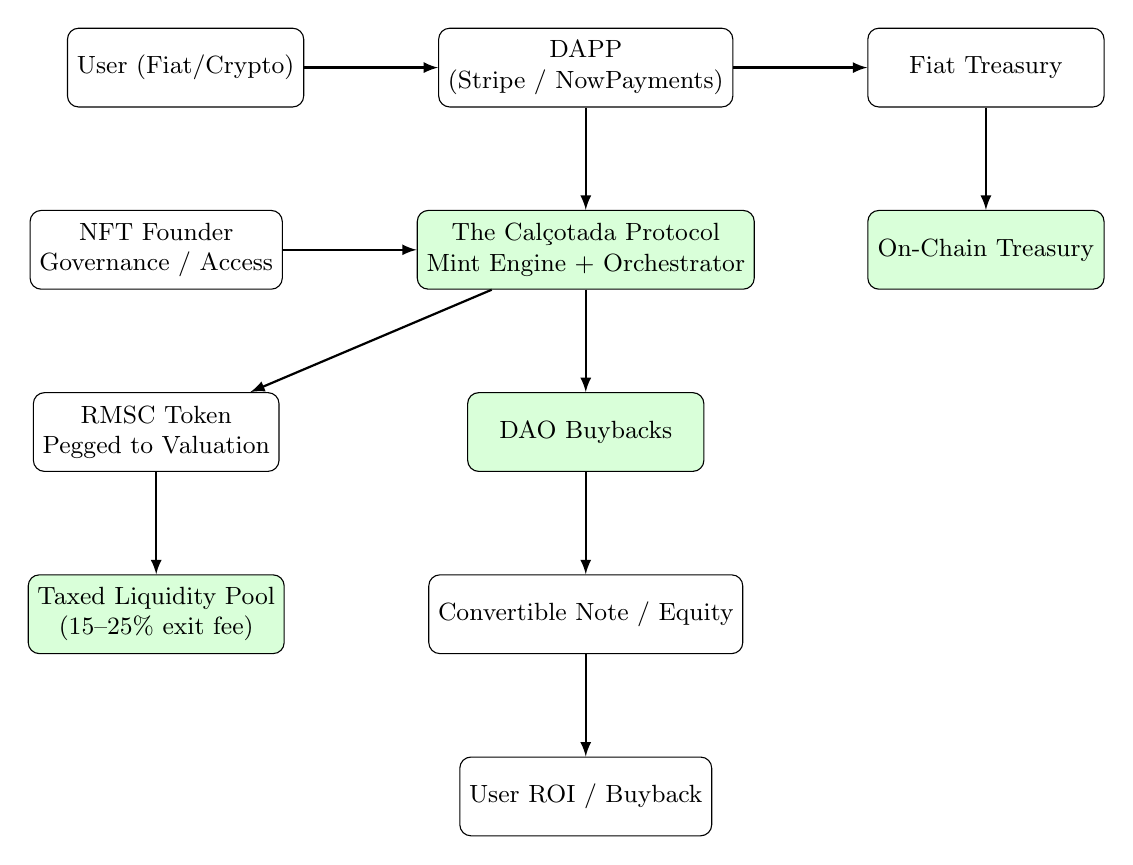
\begin{tikzpicture}[node distance=1.3cm and 1.7cm, every node/.style={font=\small}]

% Styles
\tikzstyle{box} = [draw, rounded corners, align=center, minimum width=3cm, minimum height=1cm, fill=white]
\tikzstyle{greenbox} = [box, fill=green!15]
\tikzstyle{arrow} = [->, thick, >=latex]

% Nodes
\node[box] (user) {User (Fiat/Crypto)};
\node[box, right=of user] (dapp) {DAPP\\(Stripe / NowPayments)};
\node[box, right=of dapp] (fiat) {Fiat Treasury};
\node[greenbox, below=of fiat] (onchain) {On-Chain Treasury};

\node[greenbox, below=of dapp] (protocol) {The Calçotada Protocol\\Mint Engine + Orchestrator};

\node[box, left=of protocol] (nft) {NFT Founder\\Governance / Access};
\node[box, below=of nft] (rmsc) {RMSC Token\\Pegged to Valuation};

\node[greenbox, below=of protocol] (dao) {DAO Buybacks};
\node[box, below=of dao] (equity) {Convertible Note / Equity};
\node[box, below=of equity] (payback) {User ROI / Buyback};

\node[greenbox, below=of rmsc] (tlp) {Taxed Liquidity Pool\\(15–25\% exit fee)};

% Arrows
\draw[arrow] (user) -- (dapp);
\draw[arrow] (dapp) -- (fiat);
\draw[arrow] (fiat) -- (onchain);
\draw[arrow] (dapp) -- (protocol);

\draw[arrow] (nft) -- (protocol);
\draw[arrow] (protocol) -- (rmsc);
\draw[arrow] (protocol) -- (dao);
\draw[arrow] (dao) -- (equity);
\draw[arrow] (equity) -- (payback);
\draw[arrow] (rmsc) -- (tlp);

\end{tikzpicture}%
}%
\caption{Simplified architecture of the Calçotada Protocol: dual-token issuance and treasury-integrated valuation peg.}
\end{figure}


The Calçotada Protocol implements a sophisticated two-asset system deployed on the Polygon blockchain to facilitate decentralized venture funding. The architecture consists of four core smart contracts that work in concert: CalcotCoin (NFT), Romesco (RMSC token), Calçotada (orchestrator), and NormalizeToEuro (oracle integration). This system combines governance through non-fungible tokens (NFTs) with economic participation via fungible tokens (RMSC) that are designed to track company valuation.

\subsection{CalcotCoin NFT: Governance and Foundational Access}

\begin{figure}[ht]
\centering

\includegraphics[width=0.3\textwidth]{calcot-coin-logo.png}
\caption{Calçot-Coin (CEBA) - The NFT representing community participation and governance}
\label{fig:calcotcoin-logo}
\end{figure}

The \textit{CalcotCoin} (CEBA) contract implements an ERC721 NFT system designed to recognize early supporters and provide governance rights. The current implementation features:

\textbf{Technical Specifications:}
\begin{itemize}
    \item Token Type: NFT (ERC721)
    \item Token Name: Calçot-Coin
    \item Token Symbol: CEBA
    \item Batch: 0 (Genesis)
    \item Fixed supply of 333 NFTs (CEBA Genesis edition)
    \item Public allocation: 300 NFTs
    \item Premint - Reserved Treasury: 33 NFTs
    \item Linear pricing mechanism from 222.22 to 200 RMSC per NFT
    \item Sell Price: €100 per NFT with dynamic RMSC conversion
\end{itemize}

\textbf{Minting Mechanism:}
The CalcotCoin contract implements a sophisticated dual-minting system where NFT purchases trigger a 2x RMSC mint. When purchasing an NFT:
\begin{enumerate}
    \item The buyer receives 2x the NFT price in newly minted RMSC
    \item Half of the RMSC is automatically transferred to the treasury as payment
    \item The buyer retains the other half as a bonus incentive
    \item The NFT is minted to the buyer's address
\end{enumerate}

\textbf{Planned Governance Features:}
\begin{itemize}
    \item One vote per wallet (implementation pending)
    \item Participation in valuation recognition and capital allocation decisions
    \item Access to exclusive founder communications
\end{itemize}

Note: The whitepaper originally specified 6 batches totaling 5,888 NFTs. The current implementation focuses on the initial 333-unit genesis collection, with future batches to be deployed based on protocol evolution and community feedback.

\subsection{RMSC Token: Equity-Pegged Financial Instrument}

\begin{figure}[ht]
\centering

\includegraphics[width=0.3\textwidth]{rmsc_logo.png}
\caption{Romesco (RMSCU) - The fungible token representing the "secret sauce" of venture returns}
\label{fig:rmsc-logo}
\end{figure}

The \textit{Romesco Token (RMSC)} is the core financial instrument of the protocol, implemented as an ERC20 token with ERC1363 and ERC20Permit extensions for enhanced functionality.

\textbf{Technical Implementation:}
\begin{itemize}
    \item Token Type: FT (ERC20)
    \item Token Name: Romesco
    \item Token Symbol: RMSCU
    \item Fixed maximum supply of 5,000,000 RMSC (hard cap enforced in contract)
    \item Premint Treasury: 200,000 RMSC for liquidity and operational needs
    \item Base Price: €0.40 per RMSC
    \item Pausable functionality for emergency situations
    \item Permit functionality for gasless approvals
    \item ERC1363 support for single-transaction transfers and callbacks
\end{itemize}

\textbf{Economic Design:}
\begin{itemize}
    \item Minting controlled by the orchestrator contract only
    \item No burn functionality for regular users (maintains supply integrity)
    \item Designed for future buyback mechanism at €1.5–€3.0 per RMSC
    \item Starting valuation implies approximately €0.40–€0.60 per RMSC
\end{itemize}

\textbf{Integration Features:}
The RMSC token is designed for composability with DeFi protocols:
\begin{itemize}
    \item ERC20Permit enables gasless transactions and meta-transactions
    \item ERC1363 allows for advanced payment flows and automated callbacks
    \item Standard ERC20 interface ensures compatibility with all major DEXs and lending protocols
\end{itemize}

Note: The buyback mechanism mentioned in the economic design is planned for future implementation through a separate contract that will interact with the on-chain accountancy system.

\subsection{Calçotada Orchestrator: Protocol Coordination}

The \textit{Calçotada} contract serves as the central orchestrator, coordinating interactions between all protocol components:

\textbf{Core Functions:}
\begin{itemize}
    \item Manages the dual-minting mechanism for NFT purchases
    \item Controls RMSC minting according to bonding curve pricing
    \item Handles both public and private sale mechanisms
    \item Integrates with NormalizeToEuro for multi-currency support
\end{itemize}

\textbf{Bonding Curve Implementation:}
The orchestrator implements a sophisticated normalized bonding curve using:
\begin{itemize}
    \item Q16.16 fixed-point arithmetic for precision
    \item Configurable sigmoid curve shape for optimal price discovery
    \item Integration with trapezoidal rule for accurate pricing
    \item Starting price: €0.40 per RMSC, ending price: €0.60 per RMSC
\end{itemize}

\textbf{Transaction Fee Structure:}
\begin{itemize}
    \item NFT purchases: €4.50 transaction fee
    \item RMSC purchases: €2.50 transaction fee
    \item Fees collected in POL and forwarded to treasury
\end{itemize}

\subsection{Price Oracle Integration}

The \textit{NormalizeToEuro} contract provides real-time price conversion using Chainlink oracles:

\textbf{Oracle Feeds:}
\begin{itemize}
    \item ETH/USD, EUR/USD, and POL/USD price feeds
    \item Automatic conversion between EUR pricing and POL payments
    \item 18-decimal precision for all calculations
\end{itemize}

\subsection{PEG Enforcement and Future Development}

While the current implementation provides the foundation for equity-pegged tokens, the full PEG mechanism awaits implementation:

\textbf{Current State:}
\begin{itemize}
    \item Token supply and pricing mechanisms are fully implemented
    \item Oracle integration provides real-time price conversion
    \item Treasury accumulation occurs automatically
\end{itemize}

\textbf{Planned Enhancements:}
\begin{itemize}
    \item On-chain accountancy module for transparent financial tracking
    \item Automated buyback contracts triggered by valuation milestones
    \item Governance voting mechanisms for NFT holders
    \item Integration with external valuation attestation services
\end{itemize}

\subsection{Initial Supply and Distribution}

The initial supply of RMSC tokens is allocated in a controlled and transparent manner to recognize pre-protocol contributions and prepare for public issuance. No tokens are minted speculatively or granted without capital justification.

\subsubsection{Angel Investor Allocation}

Prior to the protocol's launch, a group of early angel investors provided capital to The Calçotada Company under a convertible loan agreement. These early backers are entitled to receive RMSC tokens at the protocol’s base issuance price, plus an interest premium to account for the time value of their risk.

\begin{itemize}
    \item \textbf{Base Price Conversion:} Angel investments are converted into RMSC at the same base price offered during the initial public issuance phase.
    \item \textbf{Interest Adjustment:} A fixed 7\% interest rate is applied to the original invested amount, and this adjusted total determines the corresponding RMSC allocation.
    \item \textbf{Non-inflationary Grant:} These tokens are accounted for as part of the protocol's total capped supply and are not created in excess of the 5 million RMSC ceiling.
\end{itemize}

\subsubsection{Pre-Mint Reserve}

In addition to angel investor conversion, a total of 200,000 RMSC tokens are pre-minted and held in the protocol treasury for operational, liquidity, and market stabilization purposes. This reserve will be used judiciously to support exchange listings, liquidity pool seeding, and strategic partnerships.

\subsubsection{Public Issuance}

All remaining RMSC tokens are made available through direct, capital-backed purchase via the protocol interface. Tokens are minted on-demand as described in the Minting Scheme, with no pre-sale, airdrop, or speculative allocation.

This initial supply model ensures that token distribution is fully aligned with the company’s real financial history and avoids the common pitfalls of over-allocation, unbacked inflation, or opaque private rounds.

\subsection{Initial Distribution and Structured Pricing}

The protocol implements a sophisticated pricing mechanism that balances early adopter incentives with sustainable fundraising:

\subsubsection{Current Implementation: Genesis Collection}

The deployed contracts focus on the initial CalcotCoin Genesis collection:
\begin{itemize}
    \item 333 total NFTs with 33 reserved for treasury
    \item Linear RMSC pricing from 222.22 to 200 RMSC per NFT
    \item Fixed EUR price of €100 per NFT
    \item Dual-minting mechanism providing 2x RMSC to NFT buyers
\end{itemize}

\subsubsection{Future Batch Structure}

The protocol design accommodates future expansion through additional NFT collections:

\begin{table}[ht]
\caption{NFT Batches and Associated RMSC Minting}
\centering
\scriptsize
\begin{tabular}{|p{1.5cm}|p{0.6cm}|p{0.7cm}|p{0.7cm}|p{0.7cm}|}
\hline
\textbf{Batch} & \textbf{NFTs} & \textbf{NFT €} & \textbf{RMSC €} & \textbf{MINT kRMSC} \\
\hline
Calçot Coins     & 333  & 100  & 0.40  & 66  \\
FounderPass 1    & 555  & 125  & 0.50  & 139  \\
FounderPass 2    & 1111 & 250  & 0.525 & 529  \\
FounderPass 3    & 1111 & 375  & 0.55  & 757  \\
FounderPass 4    & 1111 & 500  & 0.575 & 966  \\
FounderPass 5    & 1111 & 625  & 0.60  & 1,157  \\
\hline
\multicolumn{5}{|c|}{\textbf{Total: 5,332 NFTs}} \\
\multicolumn{5}{|c|}{\textbf{2,047,025 € raised, 1,807,796 RMSC minted}} \\
\hline
\end{tabular}
\end{table}






Half of the RMSC minted for each NFT is transferred to the protocol treasury, while the remaining half is consumed by the NFT minting contract. This ensures that treasury-backed liquidity grows proportionally with capital raised.

\subsubsection{Public RMSC Issuance via Bonding Curve}

The Calçotada orchestrator implements a sophisticated bonding curve mechanism for public RMSC sales:

\textbf{Technical Implementation:}
\begin{itemize}
    \item Normalized sigmoid curve stored as Q16.16 fixed-point values
    \item Configurable curve shape via uploadable parameters
    \item 16-step trapezoidal integration for accurate pricing
    \item Real-time POL/EUR conversion via Chainlink oracles
\end{itemize}

\textbf{Pricing Parameters:}
\begin{itemize}
    \item Starting price: €0.40 per RMSC
    \item Ending price: €0.60 per RMSC  
    \item Available supply: Up to 4.6M RMSC (after pre-mint and NFT allocations)
    \item Transaction fee: €2.50 per purchase
\end{itemize}
\begin{figure}[ht]
\centering
\begin{tikzpicture}
\begin{axis}[
    width=\linewidth,
    height=6cm,
    grid=both,
    xlabel={\textbf{Fraction of Supply Minted}},
    ylabel={\textbf{RMSC Price (€)}},
    title={Sigmoid Bonding Curve for Public RMSC Issuance},
    ymin=39, ymax=61,
    xmin=0, xmax=1,
    thick
]
\addplot[
    color=blue,
    mark=none
]
table[
    col sep=comma,
    x=fraction_minted,
    y=rmsc_price_eur
] {rmsc_sigmoid_curve.csv};
\end{axis}
\end{tikzpicture}
\caption{Sigmoid bonding curve used for public RMSC issuance pricing.}
\label{fig:sigmoidcurve}
\end{figure}



This curve allows the protocol to capture higher marginal funding value while maintaining a predictable and fair pricing structure. Early public buyers enjoy lower prices, and late-stage buyers pay a premium as the available supply nears exhaustion.

\subsubsection{Liquidity and Secondary Market Strategy}

The protocol's liquidity strategy leverages standard DeFi infrastructure:

\textbf{Current Implementation:}
\begin{itemize}
    \item RMSC is a standard ERC20 token, compatible with all major DEXs
    \item Treasury accumulates POL and RMSC for future liquidity provision
    \item No transfer restrictions or vesting schedules
\end{itemize}

\textbf{Planned Liquidity Features:}
\begin{itemize}
    \item DEX liquidity pools on QuickSwap or Uniswap V3
    \item Treasury-funded initial liquidity provision
    \item Potential liquidity mining incentives for early providers
    \item Integration with lending protocols for RMSC collateralization
\end{itemize}

Note: The Taxed Liquidity Pool (TLP) mentioned in the original design is deferred to future protocol upgrades, allowing for simpler initial deployment and community-driven liquidity solutions.


\subsection{Network Deployment}

Polygon is selected as the base network for its:
\begin{itemize}
    \item Low transaction fees and fast confirmation times,
    \item Proven security track record via Ethereum finality,
    \item Established ecosystem of NFT and DeFi projects.
\end{itemize}

Deploying on Polygon enables frictionless user participation while ensuring composability with future liquidity protocols and DAO tools.



\section{Technical Implementation}

\subsection{Smart Contract Architecture}

The Calçotada Protocol consists of four core smart contracts deployed on Polygon:

\textbf{1. CalcotCoin.sol (ERC721):}
\begin{itemize}
    \item Manages NFT issuance and ownership
    \item Implements linear pricing mechanism
    \item Handles treasury pre-allocation
    \item Integrates with orchestrator for minting
\end{itemize}

\textbf{2. Romesco.sol (ERC20):}
\begin{itemize}
    \item Implements capped token supply (5M RMSC)
    \item Provides ERC1363 and Permit extensions
    \item Controlled minting via orchestrator only
    \item Pausable for emergency situations
\end{itemize}

\textbf{3. Calcotada.sol (Orchestrator):}
\begin{itemize}
    \item Coordinates all protocol interactions
    \item Implements bonding curve pricing
    \item Manages dual-minting mechanism
    \item Handles fee collection and treasury forwarding
\end{itemize}

\textbf{4. NormalizeToEuro.sol (Oracle):}
\begin{itemize}
    \item Integrates Chainlink price feeds
    \item Provides EUR/POL/ETH conversions
    \item Ensures accurate multi-currency pricing
\end{itemize}

\subsection{Security Considerations}

\textbf{Access Control:}
\begin{itemize}
    \item Owner-controlled administrative functions
    \item Orchestrator pattern for inter-contract calls
    \item No external minting access on token contracts
\end{itemize}

\textbf{Safety Features:}
\begin{itemize}
    \item ReentrancyGuard on all payment functions
    \item Pausable functionality for emergency response
    \item Overflow protection via Solidity 0.8.28
    \item Battle-tested OpenZeppelin libraries
\end{itemize}

\subsection{Gas Optimization}

\begin{itemize}
    \item Batch minting reduces per-NFT gas costs
    \item Q16.16 arithmetic minimizes computational overhead
    \item Efficient storage patterns in bonding curve
    \item Optimized loops with unchecked arithmetic where safe
\end{itemize}

\subsection{Protocol Composability}

The Calçotada Protocol exposes several public and payable functions that enhance composability with other DeFi protocols:

\textbf{Public Query Functions:}
\begin{itemize}
    \item \texttt{previewPurchaseCost}: Returns prices in POL for RMSC purchases
    \item \texttt{previewPurchaseCostEur}: Returns prices in EUR for RMSC purchases
    \item \texttt{getPriceBatchNFT}: Provides pricing for NFT batches in both POL and EUR
\end{itemize}

\textbf{Payable Minting Functions:}
\begin{itemize}
    \item \texttt{calcotCoinPublicMint}: Allows public minting of NFTs with POL payment
    \item \texttt{publicRmscMint}: Enables direct RMSC token purchases (not yet exposed in UI)
\end{itemize}

These functions allow external protocols and smart contracts to integrate with the Calçotada ecosystem, enabling:
\begin{itemize}
    \item Automated trading strategies based on real-time pricing
    \item Integration with DEX aggregators for optimal routing
    \item Building of derivative products on top of RMSC tokens
    \item Creation of vaults and yield strategies
\end{itemize}

\section{Vision: From Meme Coins to PEG Coins}

This whitepaper presents not just a protocol implementation, but a vision for transforming venture capital through blockchain technology. We invite builders, researchers, and visionaries to join us in developing the foundational components for true DAO-based venture capital.

\subsection{Redefining PEG: From Price Stability to Performance Growth}

The term "PEG" in traditional crypto contexts typically refers to price-pegged assets like stablecoins. We intentionally reappropriate this term to create a powerful contrast with MEME coins. While MEME coins represent pure speculation without underlying value, PEG (Performance Equity Growth) tokens represent the opposite: real value creation tied to company performance.

\textbf{The MEME vs PEG Paradigm:}
\begin{itemize}
    \item \textbf{MEME}: Speculation, hype-driven, no intrinsic value
    \item \textbf{PEG}: Performance-driven, value-backed, growth-oriented
\end{itemize}

Unlike traditional price pegs that maintain stable values, our PEG tokens are \textit{pegged to company growth}. This represents a new category of crypto assets:
\begin{itemize}
    \item Not pegged to a stable price (like USDT to USD)
    \item Not pegged to another asset (like WBTC to BTC)
    \item But pegged to a company's valuation trajectory and success
\end{itemize}

This redefinition serves a dual purpose: it creates a memorable contrast with MEME coins while accurately describing tokens that track real business performance. PEG tokens offer the excitement of venture returns with the substance of equity participation—transforming speculation into investment.

\subsection{The Composability Foundation}

The Calçotada Protocol aims to establish standardized components that any startup can use to create their own equity-pegged tokens:

\textbf{Standardized Valuation Methods:}
We propose using Discounted Cash Flow (DCF) models as the industry standard for early-stage startup valuations. Unlike traditional approaches, our innovation embeds buyback mechanisms directly tied to current company performance. This creates a new standard where:
\begin{itemize}
    \item Valuations are calculated transparently on-chain
    \item External parameters (industry multipliers, WACC) are provided by oracles
    \item Buybacks are triggered automatically based on performance milestones
    \item Early liquidity is provided through a SAFE + Interest model
\end{itemize}

\textbf{Projected Returns (2027-2032):}
Based on our DCF models for The Calçotada Company:
\begin{itemize}
    \item Pessimistic scenario: 2.1x return by 2031
    \item Standard scenario: 2.8x return by 2031
    \item Optimistic scenario: 5.5x return by 2031
\end{itemize}

\subsection{On-Chain Accountancy Revolution}

Current accounting depends on centralized bank integrations and proprietary software. We envision:
\begin{itemize}
    \item Immutable, auditable financial records on-chain
    \item Access to real-time Free Cash Flow data
    \item New ecosystem of accountancy DApps
    \item Smart contract auditors guaranteeing transparency
    \item Integration with privacy solutions (e.g., Hyperledger) for competitive data
\end{itemize}

\subsection{Capturing the Meme Coin Market}

The crypto community investing in meme coins represents untapped potential for meaningful investments:

\textbf{What PEG Coins Offer:}
\begin{itemize}
    \item High risk/reward profile similar to meme coins
    \item 20\% early rewards for liquidity providers
    \item Long-term returns ranging from 2x to 5.5x
    \item Real utility backing token value
    \item Community engagement through governance
\end{itemize}

\textbf{Liquidity Strategy:}
\begin{itemize}
    \item Early liquidity pools with tax mechanisms for flippers
    \item Rewards for long-term believers
    \item Transition from speculation to value creation
\end{itemize}

\subsection{Building Trust Through Standards}

The protocol addresses fundamental trust barriers:
\begin{itemize}
    \item \textbf{Valuation Trust:} Pre-defined DCF models with oracle-provided parameters
    \item \textbf{Buyback Trust:} Smart contract execution with public reserves
    \item \textbf{Process Trust:} Deterministic mathematical expressions
    \item \textbf{Access Trust:} Guaranteed participation in seed capital opportunities
\end{itemize}

\subsection{Target Audience and Growth}

\textbf{Primary Targets:}
\begin{itemize}
    \item Retail investors currently in meme coins seeking real utility
    \item Young professionals interested in startup investing
    \item International investors excluded from traditional VC
    \item Non-accredited investors seeking early-stage opportunities
\end{itemize}

\textbf{Growth Mechanisms:}
\begin{itemize}
    \item Referral system (5 RMSC per new user)
    \item Education initiatives on equity pegs
    \item Community-driven protocol development
\end{itemize}

\subsection{Five-Year Success Metrics}

By 2029, success means:
\begin{itemize}
    \item The Calçotada Company operating at full scale in Europe
    \item 3 patents published on protocol innovations
    \item Profitable operations from year 3
    \item Active buyback program demonstrating model viability
    \item RMSC accepted as collateral in major DeFi protocols
    \item Establishment of the "Calçotada Standard" for equity pegs
\end{itemize}

\subsection{Call for Builders and Contributors}

This whitepaper is a proposal and invitation. We seek:
\begin{itemize}
    \item \textbf{Protocol Developers:} To build standardized components
    \item \textbf{Oracle Integrators:} To validate fiat transactions
    \item \textbf{Financial Engineers:} To refine DCF models
    \item \textbf{Legal Experts:} To navigate regulatory frameworks
    \item \textbf{Community Leaders:} To educate and onboard users
    \item \textbf{Startup Founders:} To adopt and test the protocol
\end{itemize}

Many questions remain unanswered—optimal update frequencies, discount rates for pre-revenue startups, governance structures. These will be defined collectively as we build this new foundation for venture capital.

The Calçotada Protocol is more than technology; it's a movement toward democratized, transparent, and accessible startup funding. Join us in creating the future of venture capital.

\section{The Calçotada Company: Protocol Sponsor}

\subsection{Company Overview}

The Calçotada Company is a Barcelona-based food-tech startup pioneering Food Experience as a Service (FEaaS). As the primary sponsor and first implementation of the Calçotada Protocol, the company serves as both a proof of concept and a real-world test case for tokenized venture funding.

\subsection{Business Model: FEaaS}

Food Experience as a Service (FEaaS) represents a paradigm shift in the hospitality industry:

\begin{itemize}
    \item \textbf{Scalable Culinary Experiences:} Transforming traditional dining into reproducible, high-quality experiences
    \item \textbf{Technology-Enabled Operations:} Leveraging automation and data analytics to optimize food service
    \item \textbf{Franchise-Ready Model:} Creating standardized processes that maintain authenticity while enabling rapid expansion
    \item \textbf{Cultural Preservation:} Protecting and promoting traditional Catalan cuisine through modern business practices
\end{itemize}

\subsection{Why Calçotada?}

The company takes its name from the traditional Catalan calçotada—a communal feast celebrating spring onions. This choice reflects:
\begin{itemize}
    \item Community-driven values aligned with DAO principles
    \item Scalable social experiences perfect for FEaaS model
    \item Strong cultural identity providing market differentiation
    \item Natural alignment between shared meals and shared ownership
\end{itemize}

\subsection{Protocol Synergy}

The Calçotada Company's use of the protocol demonstrates:
\begin{itemize}
    \item Real revenue generation for buyback mechanisms
    \item Clear valuation metrics through operational data
    \item Community engagement through product and investment
    \item Bridge between physical business and digital assets
\end{itemize}

\section{Team and Acknowledgments}

The Calçotada Protocol is driven by a dedicated team of RMSC holders representing the company's interests:

\textbf{Dr. Julià Delos Ayllón} - Founder and Chief Architect. With a distinguished career spanning from software to high-power systems, Dr. Ayllón holds a PhD in Electrical Engineering focused on power electronics and LED driver optimization. His professional journey includes roles at Philips Research, HP, and Lear Corporation, where he developed innovative solutions from embedded software to advanced power management systems. At Philips Research, he contributed to multiple patents in LED driver technology and integrated power systems. This deep technical expertise in hardware miniaturization and system optimization now informs his approach to blockchain protocol design. Dr. Ayllón founded The Calçotada Company with a vision to revolutionize access to food experiences through a Food Experience as a Service (FEaaS) business model—creating an "Airbnb for culinary experiences" that enables rapid scaling while preserving authentic local gastronomy. His unique background bridges hardware engineering, corporate R\&D, and entrepreneurial innovation, positioning him to architect protocols that merge real-world business models with decentralized finance.

\textbf{Dr. Louisa Spaans} - Medical doctor and protocol keyguard. Early angel investor and major RMSC holder safeguarding protocol integrity.

\textbf{Dr. Dimitri Pustakhod} - PhD and protocol keyguard. Strategic advisor and major RMSC holder ensuring governance alignment.

\textbf{Danail Hristov} - Telecom engineer and protocol keyguard. Technical advisor and major RMSC holder protecting protocol development.

This team represents the convergence of technical innovation, medical precision, business acumen, and entrepreneurial vision—united in democratizing access to venture capital through blockchain technology.

\section{Conclusion and Future Work}

The Calçotada Protocol represents a significant step toward democratizing venture capital through blockchain technology. By implementing tokenized convertible notes with clear valuation pegs, the protocol creates a bridge between traditional startup funding and decentralized finance.

\subsection{Current MVP Implementation}

The deployed Minimum Viable Product serves as a proof of concept and market validation tool:

\textbf{Implemented Features:}
\begin{itemize}
    \item Genesis collection of 333 CalçotCoin NFTs at €100 each
    \item RMSC token with 5M supply cap and bonding curve mechanics
    \item Dual-minting system rewarding early supporters
    \item Oracle integration for EUR/POL price conversion
    \item Basic treasury accumulation mechanism
\end{itemize}

\textbf{MVP Objectives:}
\begin{itemize}
    \item Demonstrate technical feasibility of tokenized venture funding
    \item Validate market demand with €30,000 initial raise target
    \item Build initial community of supporters and advisors
    \item Test smart contract security and gas efficiency
    \item Establish foundation for future protocol development
\end{itemize}

This MVP represents a testimonial to the work ahead, starting with a solid foundation of minting strategies and bonding curve sales mechanisms. The limited scope allows for careful iteration based on community feedback before expanding to the full protocol vision.

\subsection{Development Roadmap}

The current deployment represents a Minimum Viable Product (MVP) designed to validate market interest and establish the foundational infrastructure. The roadmap prioritizes sustainable growth and community building over rapid feature deployment.

\textbf{Whitepaper Publication and Protocol Launch:}
This whitepaper will be released concurrently with the public announcement of the Calçotada Protocol, marking the official start of Phase 1.

\textbf{Phase 1 - MVP Validation and Team Formation (Current - Q3 2024):}
\begin{itemize}
    \item Target: Raise initial €30,000 through Genesis collection (333 NFTs)
    \item Validate market interest and protocol mechanics
    \item Build core team for protocol development
    \item Present protocol to major blockchain networks and communities
    \item Establish fundamental protocol standards
    \item Define trustworthy governance framework
\end{itemize}

\textbf{Phase 2 - Protocol Expansion (Q4 2024 - 2025):}
\begin{itemize}
    \item Launch second NFT collection (September 2024 target)
    \item Release full 5,555 NFT collection based on community feedback
    \item Define operational phases for The Calçotada Company
    \item Establish protocol update and governance strategies
    \item Begin development of on-chain accountancy framework
\end{itemize}

\textbf{Phase 3 - Operations Launch (2025-2026):}
\begin{itemize}
    \item Calçotada Company begins operations with collected funds
    \item First products delivered to market
    \item Protocol provides initial company valuation estimates
    \item Deploy liquidity pools on major DEXs
    \item Implement basic financial reporting on-chain
\end{itemize}

\textbf{Phase 4 - Value Realization (2027+):}
\begin{itemize}
    \item Initiate first buyback programs based on company profits
    \item Define and communicate exit strategies for token holders
    \item Expand protocol to support additional portfolio companies
    \item Establish Calçotada Protocol as standard for tokenized venture funding
\end{itemize}

\subsection{Research Directions}

Future research will explore:
\begin{itemize}
    \item Optimal bonding curve parameters for different funding stages
    \item Integration of zero-knowledge proofs for private financial data
    \item Cross-chain implementations for broader accessibility
    \item Regulatory compliance frameworks for security token standards
\end{itemize}

The Calçotada Protocol MVP demonstrates the technical feasibility of tokenized venture funding while prioritizing community validation and sustainable growth. By starting with a focused Genesis collection of 333 NFTs, the protocol seeks to validate market interest, build a dedicated team, and establish fundamental standards before expanding to its full vision. This measured approach ensures that when the protocol scales to support The Calçotada Company's operations and eventual buybacks, it will do so with proven mechanics, community trust, and a clear path to delivering value to all stakeholders. The journey from MVP to full protocol implementation represents not just a technical roadmap, but a new model for inclusive, transparent venture capital.


\appendix
\section{Cultural Inspiration: The Calçotada Tradition}

We'll be the first to admit it: a blockchain protocol named after a charred onion is unusual. But a \textit{calçot} is no ordinary onion. When grilled over an open flame, its outer layers burn away to reveal a heart of astonishingly sweet, tender deliciousness, perfect for dipping in a rich romesco sauce. The Calçotada Protocol draws its name from this Catalan tradition of \textit{la calçotada}, a communal feast that embodies shared effort and collective success—values we believe mirror our mission to democratize access to venture capital.

Beyond the symbolism, the names are a bit of fun that links the protocol directly to its sponsoring entity, \textbf{The Calçotada Company}. We believe that the success of our fundraising will bring us all a step closer to earning a seat at a real \textit{calçotada} feast. It's a culinary reward for a financial breakthrough.

The protocol's dual-token architecture reflects this heritage:
\begin{itemize}
    \item \textbf{The NFT (Calçot-Coin)}: Represents governance and participation. NFT holders are part of the decision-making collective, with voting rights and access to benefits as the company and protocol grow. This also guarantees participation in yearly meetings to try and enjoy the company’s products. The NFTs are freely tradable, and holders will have founding advantages in financing and the use of services.
    \item \textbf{The RMSC Token (Romesco)}: Represents capital and returns. The freely tradable RMSC token is designed to capture company performance while remaining detached from governance, preventing the concentration of influence among large holders. The secret, after all, is in the sauce.
\end{itemize}

Ultimately, retaining these names provides a distinctive, culturally resonant identity, reinforcing the connection between the protocol and The Calçotada Company, and ensuring brand consistency and long-term visibility.
\bibliographystyle{IEEEtran}
\bibliography{references}

\end{document}
